

%
% Chapter 6
%

\chapter{TIME DIVISION DUPLEX SYSTEM}
\label{chap:TDD}
As discussed in Chapter \ref{chap:strategyAnalysis}, feedback is incorporated into our strategies. This chapter focuses on the implementation of TDD with USRP and GNU Radio.

\begin{figure}[tpb]
  \begin{center}
    \centerline{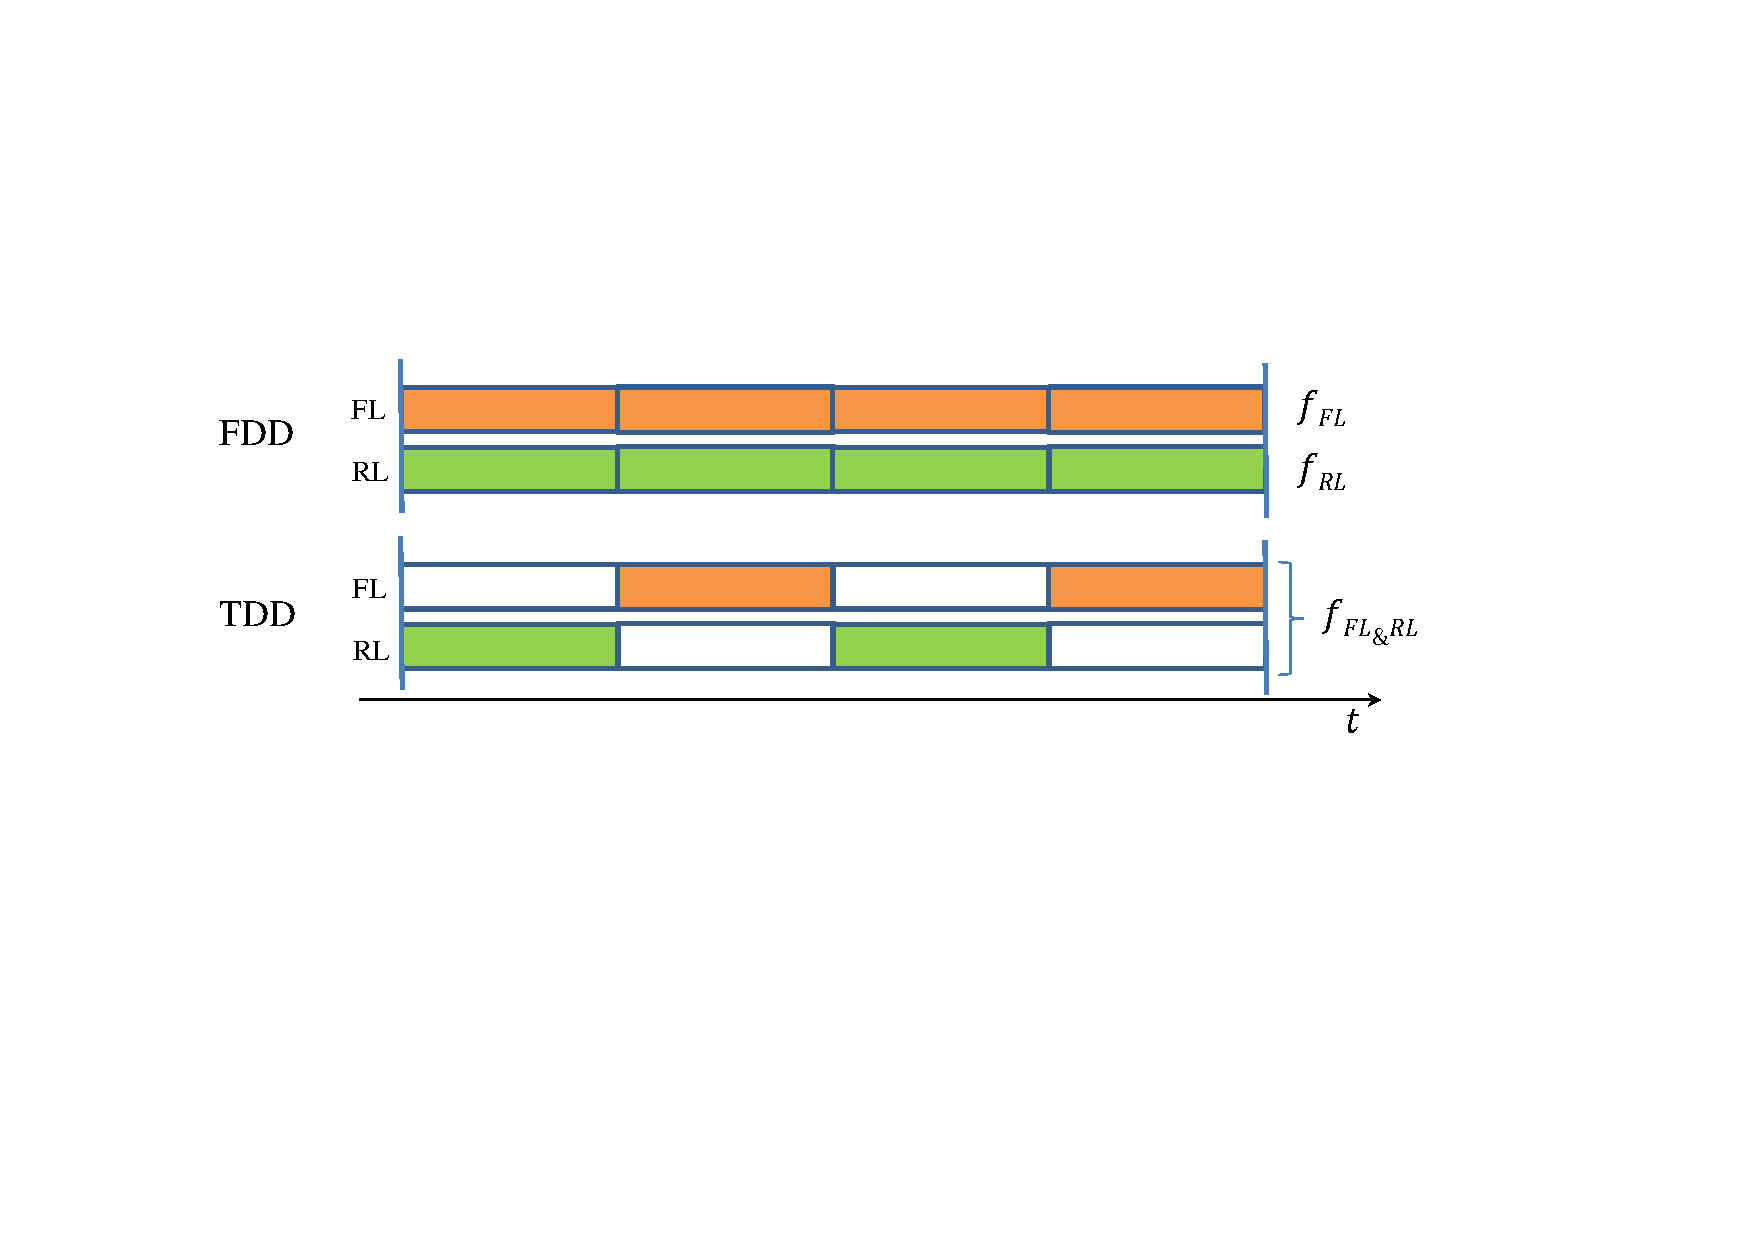
\includegraphics[width=140mm]{TDDandFDD.pdf}}
    \caption{Illustration of TDD and FDD. FL stands for forward link, and RL stands for reverse link.}
    \label{fig:TDDandFDD}
  \end{center}
\end{figure}

\section{Introduction to TDD}
In the TDD method, a single frequency band is assigned to both the transmitter and the receiver, and the forward link and reverse link use the same spectrum at different times as shown in Figure~\ref{fig:TDDandFDD}. There are some advantages of TDD over FDD \cite{MoonbLinkTDDFDD}:
\begin{itemize}

\item In TDD, a guard band is not required to separate the forward link and reverse link. However, a guard time is necessary for synchronization purposes. Generally, the spectrum cost of the guard time is less than that of the guard band in FDD in terms of spectrum efficiency.

\item In TDD, only one set of parameters or one physical layer is needed, because of the symmetry of forward link and reverse link. However, in FDD, two sets of parameters have to be tuned for both links or two physical layers have to be developed for each link.

\item The TDD scheme can dynamically allocate the proportion of time slots assigned to forward link and reverse link while it is difficult for FDD implementations to dynamically adjust the proportion of spectrum usage for both links.
\end{itemize}

Examples of technologies using TDD include Universal Mobile Telecommunications System (UMTS) 3G supplementary air interfaces, TD-CDMA for mobile telecommunications, TD-SCDMA 3G mobile telephony air interface, Chinese TD-LTE 4G and TD-SCDMA 3G mobile communications, DECT wireless telephony, IEEE 802.16 WiMAX, PACTOR, and digital enhanced cordless telecommunications (DECT) wireless telephony \cite{wikipediaDuplex, TechoPediaTDD}.

\section{Design and Implementation of TDD System}
In a TDD system, the key issue is the time synchronization between source and destination. To achieve good synchronization, the transmission time and receiving time for both the source and destination should be controlled. The USRP N210 has a mode called burst mode that can be used to control the transmission time. In software, stream tags in GNU Radio are used to control the burst mode of USRP.
\subsection{Introduction to Stream Tags and USRP Burst Mode}
A stream tag is an isosynchronous data stream that runs parallel to the main data stream in GNU Radio \cite{GNURadioStreamTags}. A stream tag can be generated by a signal processing block and can be attached to a particular data sample. The stream tag moves along with the data sample to the following blocks until it reaches a sink block or is forced to stop propagating by another signal processing block, which can be set up by the programmer.

A stream tag consists of a key, a value, and a source ID. The key identifies the type of information inside the streams tag. The value is the message carried by the stream tag. The source ID defines the name of the block creating the stream tag. The key, value, and source ID are all PMTs (Polymorphic Types) defined in GNU Radio. In practice, the type can be used to store anything, and it also has simple conversion methods for common data types such as boolean, long, or vector in C++. For details of PMTs, please refer to \cite{GNURadioPolymorphicType}.

Each data processing block can call a GNU Radio system function to read all of the stream tags contained in incoming samples. The block can identify the stream tags by their source ID and key.

USRP Burst Mode can be controlled by three tags with fixed keys, defined by the USRP hardware and GNU Radio software, which are \texttt{tx\_time}, \texttt{tx\_sob} and \texttt{rx\_sob} defined by USRP and GNU. The value of the \texttt{tx\_time} stream tag defines the start time of the first data sample in a burst transmission round. The start time is the USRP time maintained in the USRP hardware and counted in seconds from  the instant that the USRP is powered on. The \texttt{tx\_sob} tag orders the USRP transmitter to be in burst mode starting with the next data sample, and the \texttt{rx\_sob} stream tag tells the USRP transmitter to stop burst mode and to switch to normal transmission mode with the next data sample.

Another system stream tag defined by USRP and GNU Radio is \texttt{rx\_time}, which tells the USRP time at which the sample is sent from the USRP to the GNU Radio through the Ethernet interface. It is sent only once for the first data sample when system just starts or overflow happens. Overflow is unique to the software receiver. When overflow occurs, the processing speed of the host PC cannot keep up with the received data from the USRP. Consequently, the buffer in the USRP overflows, and the data samples are dropped. The stream tag \texttt{rx\_time} is very helpful for the implementation of a TDD system, which will be explained in the following section.

\subsection{Tagger and Muter}
As shown in Figure \ref{fig:MuterTaggerFlowgraph}, GNU Radio signal processing blocks called Tagger and Muter have been developed to control the TDD operation. The Tagger manages the burst transmission, and the Muter decides whether data samples are forwarded to the following blocks based on the TDD state. The Muter also keeps track of the USRP time at the GNU Radio software level.

\begin{figure}[tpb]
  \begin{center}
    \centerline{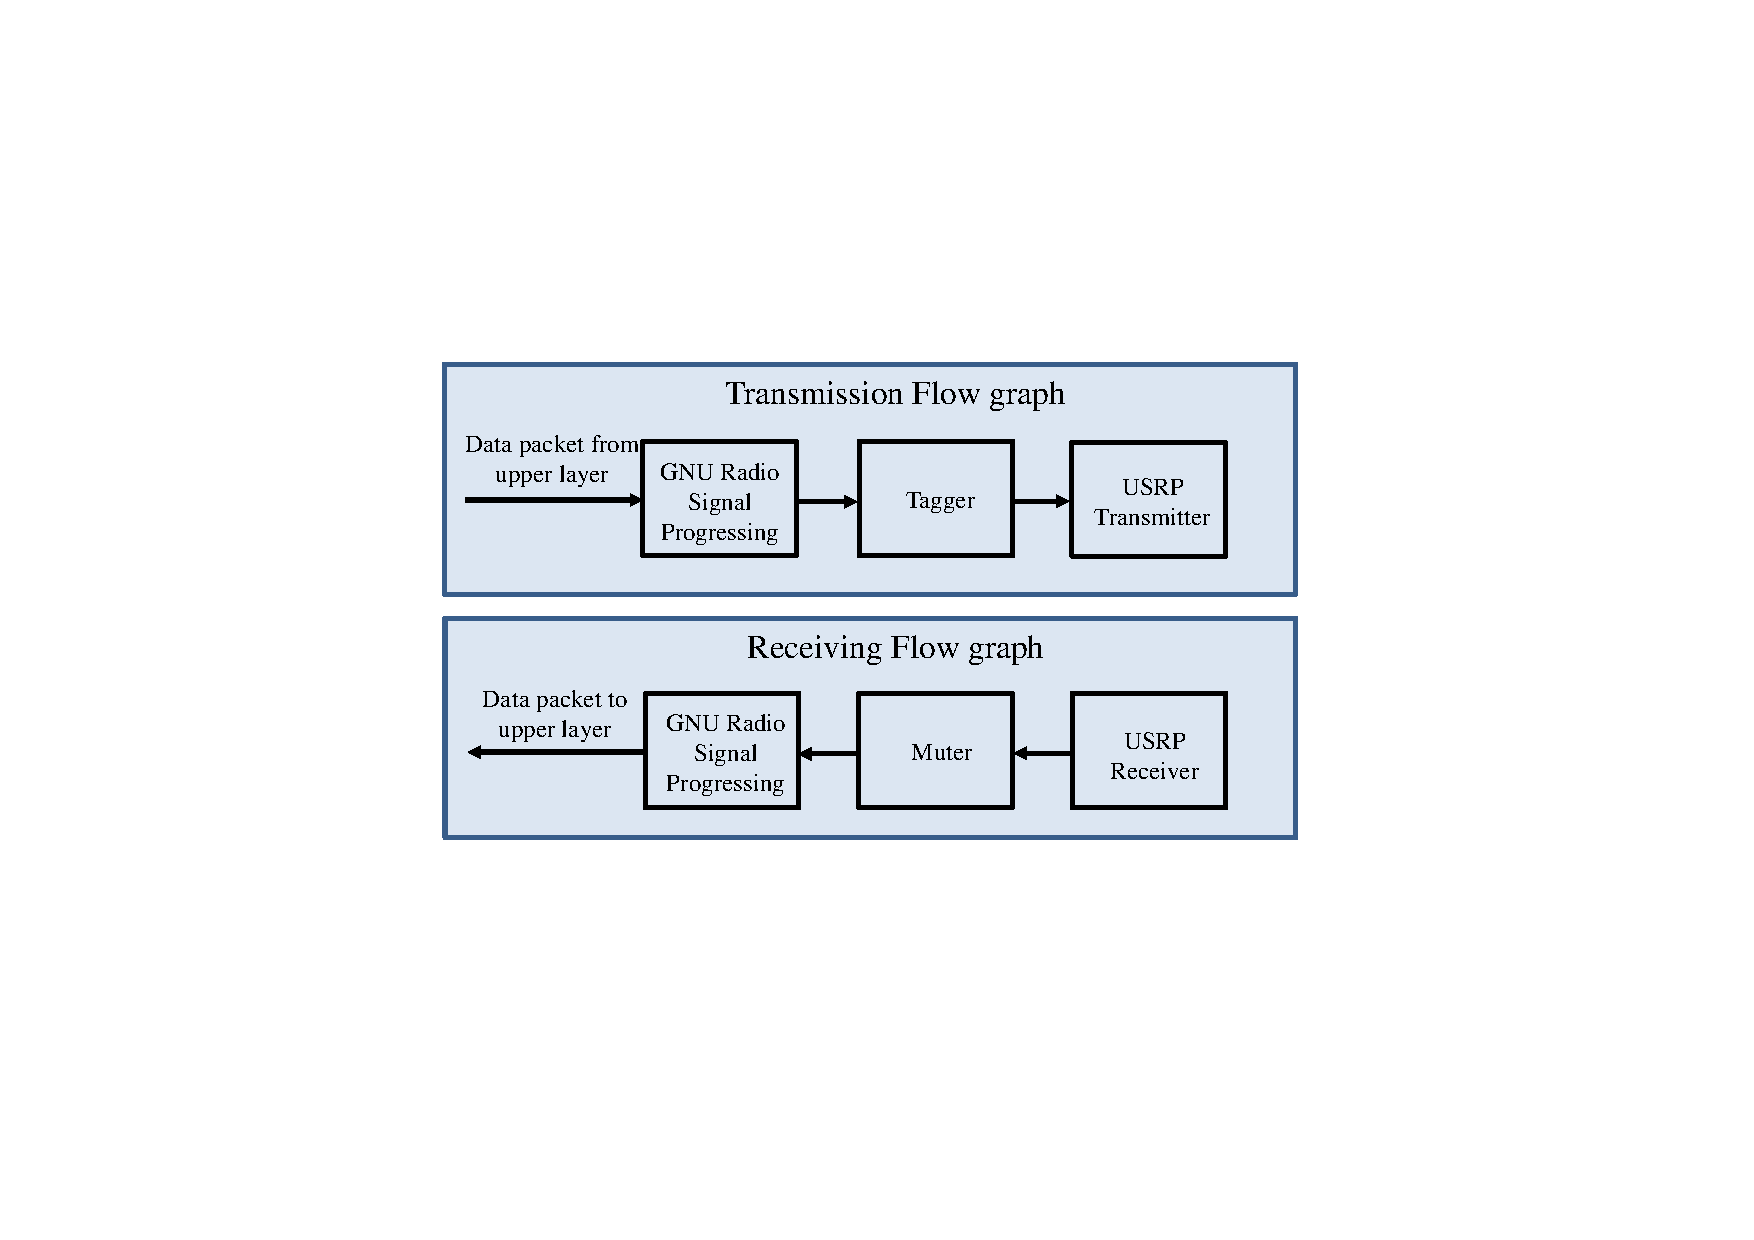
\includegraphics[width=140mm]{MuterTaggerFlowgraph.pdf}}
    \caption{Tagger and Muter in the transmission and receiving flow graphs.}
    \label{fig:MuterTaggerFlowgraph}
  \end{center}
\end{figure}

\subsubsection{Tagger}
The Tagger controls the burst transmission by stream tags \texttt{tx\_time}, \texttt{tx\_sob} and \texttt{rx\_sob}. Let the idle period be the receiving period of a TDD cycle and define the idle duration to be the time of an idle period. The Tagger calculates the idle duration and the burst duration based upon the number of samples from prior blocks and the sampling rate of the USRP, e.g., 5 MHz.

During system initialization, an upper layer function obtains the USRP time through the function \texttt{get\_time\_now}, and sets an initial burst time based on the current USRP time. The Tagger then automatically updates the next burst time based on the calculated idle and burst durations. There is also an interface in Tagger to receive adjusted burst times from the Muter so that the TDD burst cycle can be dynamically adjusted.
\subsubsection{Muter}
The Muter connects directly to the USRP source block. There is a software clock in Muter to keep track of the USRP time. The Muter waits for the \texttt{rx\_time} tag. Once it receives a \texttt{rx\_time} tag, the Muter will update its software clock time to the USRP time contained in the stream tag, which we will denote as $t_s$. The Muter will continue to update its clock based on $t_s$, the number of samples received after the tag ($N_S$), and the sampling rate ($R_S$), according to
\begin{align}
{t_c} = {t_s} + \frac{{{N_S}}}{{{R_S}}}.
\end{align}

The Muter controls each TDD cycle with an estimate of the USRP hardware time by forwarding and blocking data samples at the appropriate time. In an operation defined as Disable Muter, the Muter forwards the data samples to next signal processing block in the receiving mode. In the complementary operation defined as Enable Muter, the Muter blocks the data samples in transmission mode by setting the received data samples to be 0, which prevents receiving data sent from the same antenna.

A TDD sub-frame, and a physical-layer packet have been defined in Section \ref{comptititveStrategy}. Each sub-frame requires 1.74 milliseconds to transmit. In the header of every reverse link physical-layer packet, there is one byte called ``sub-frame'' left indicating how many TDD sub-frames remain in the current receiving mode in a TDD cycle. The Muter can adjust its samples that need to be forwarded in the current Muter enabling state.

However, signal processing delay occurs from the time a physical-layer packet is received in the Muter to the time the ``sub-frame left'' information is decoded and passed to the Muter. The delay can be estimated in the physical layer. The Muter adds stream tags containing the current USRP time in the data samples. After the physical-layer packet has been decoded, the physical layer obtains the current USRP time from the Muter and compares it with the time contained in the stream tags to calculate the packet processing delay. The calculated delay is passed to the Muter. Then the Muter can adjust the TDD cycle based on the ``sub-frame left'' information and the signal processing delay. At the same time, the Muter can also calculate the next start time of a burst transmission and pass it to the Tagger. The Tagger will adjust its next start time accordingly.

The TDD timing adjustment feature of the Muter can be set to be ON or OFF.

\subsection{Two-way TDD Timing Adjustment vs. One-way TDD Timing Adjustment}
In GNU Radio and the USRP, if the data has been pushed to the buffer in the USRP, its burst time cannot be changed. Therefore, the data in the next burst transmission has to be prepared in advance. There is also variable signal processing time and Ethernet transmission time in the GNU Radio and USRP. A typical value would be several milliseconds. As a result, the burst data needs to be prepared one TDD cycle ahead of the burst start time.

Suppose a TDD cycle starts with the receiving period. The timing adjustment in the Muter is in effect immediately while the timing adjustment in the Tagger will not be in effect until next TDD cycle, because the burst data in the current TDD cycle has been sent to the USRP and cannot be changed.

Ideally, two-way TDD timing adjustment is preferable. However, the preparation of burst data in advance makes this impossible. Figure \ref{fig:TDDtwoWayAdjustment} shows an example of two-way TDD timing adjustment. Guard time is not considered here. Suppose that starting from time $t_0$, the timing of the destination has a $\Delta t$ offset with respect to the source. Then the adjustment scheme starts to work. However, from $t_1$ to $t_2$, the adjustment does not fulfill a good synchronization between the source and destination. Actually, the adjustment process will just repeat the situation from $t_1$ to $t_2$ forever. Consequently, two-way TDD timing adjustment fails.


\begin{figure}[tpb]
  \begin{center}
    \centerline{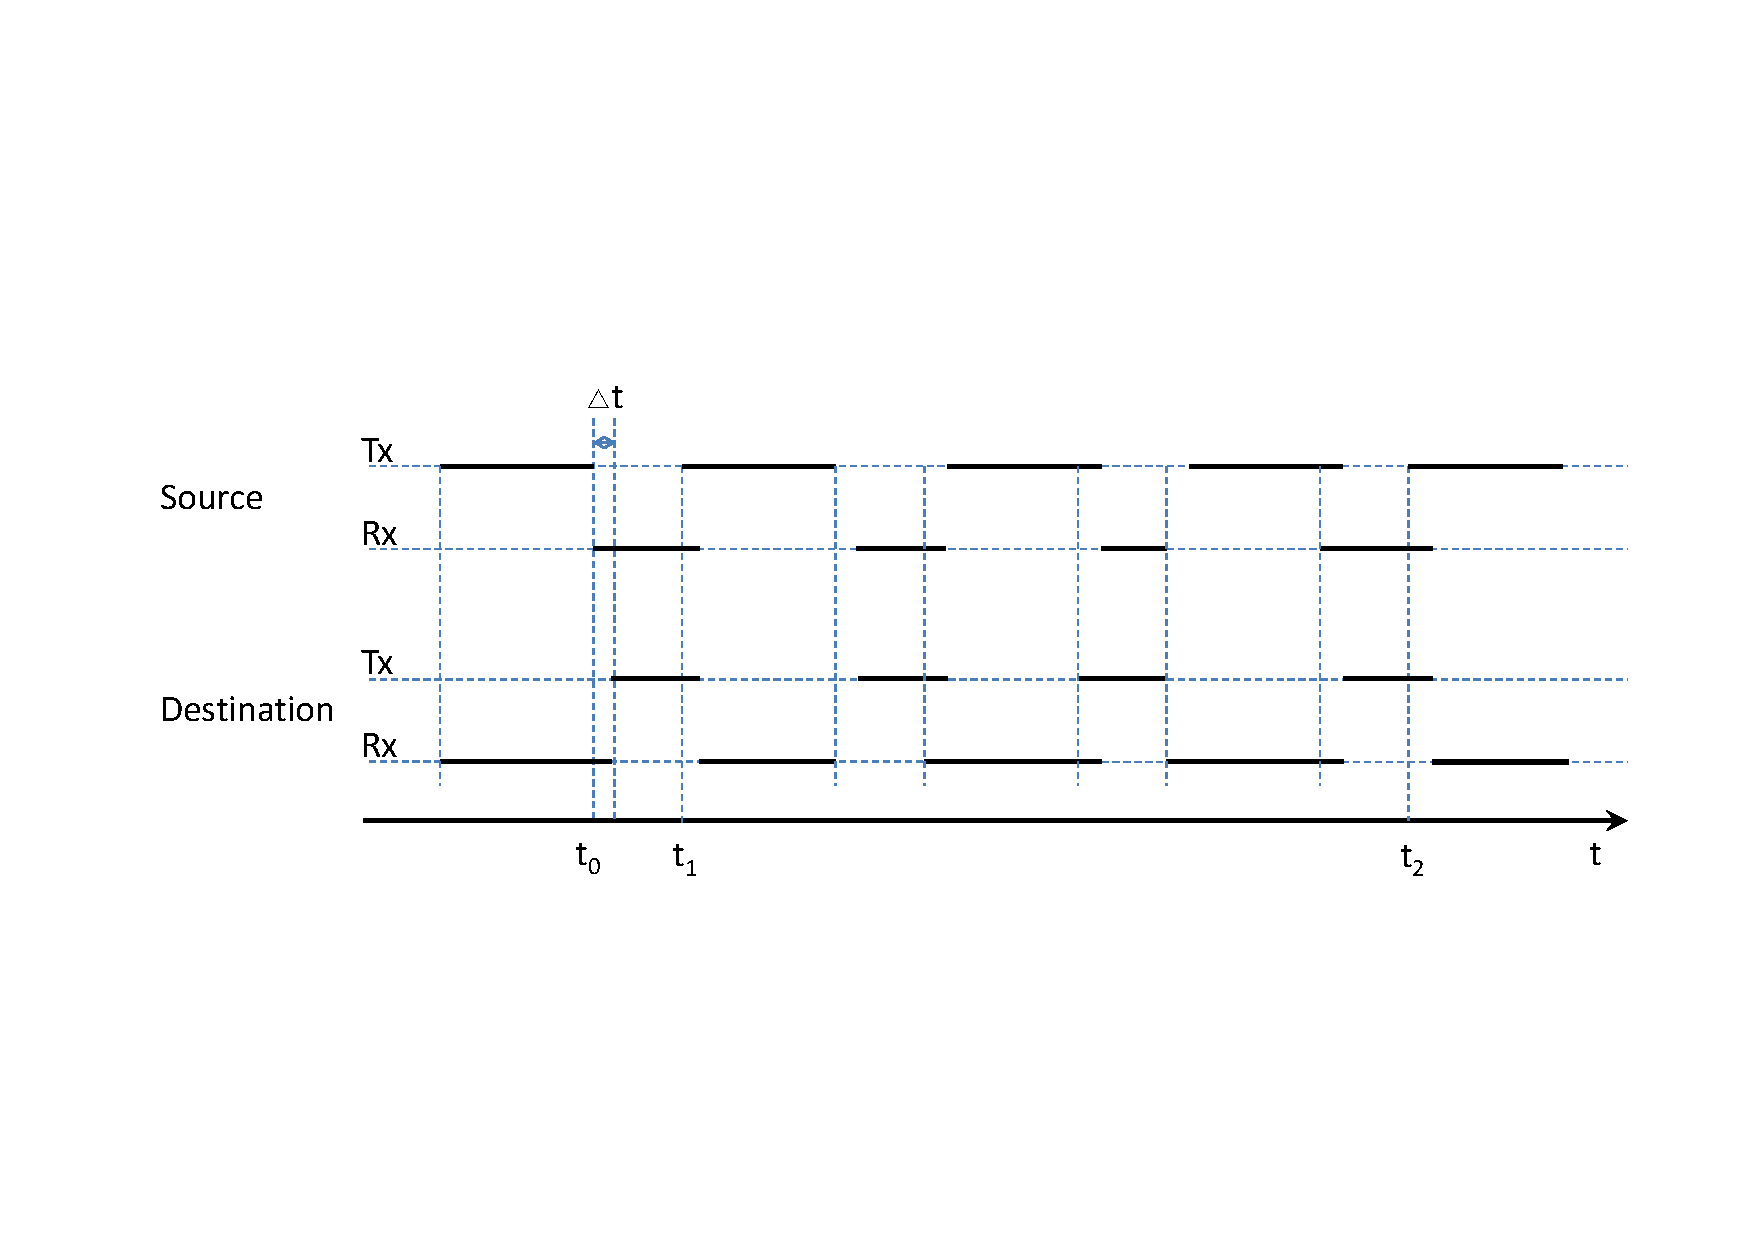
\includegraphics[width=160mm]{TDDtwoWayAdjustment.pdf}}
    \caption{Example of two-way TDD timing adjustment.}
    \label{fig:TDDtwoWayAdjustment}
  \end{center}
\end{figure}


\begin{figure}[tpb]
  \begin{center}
    \centerline{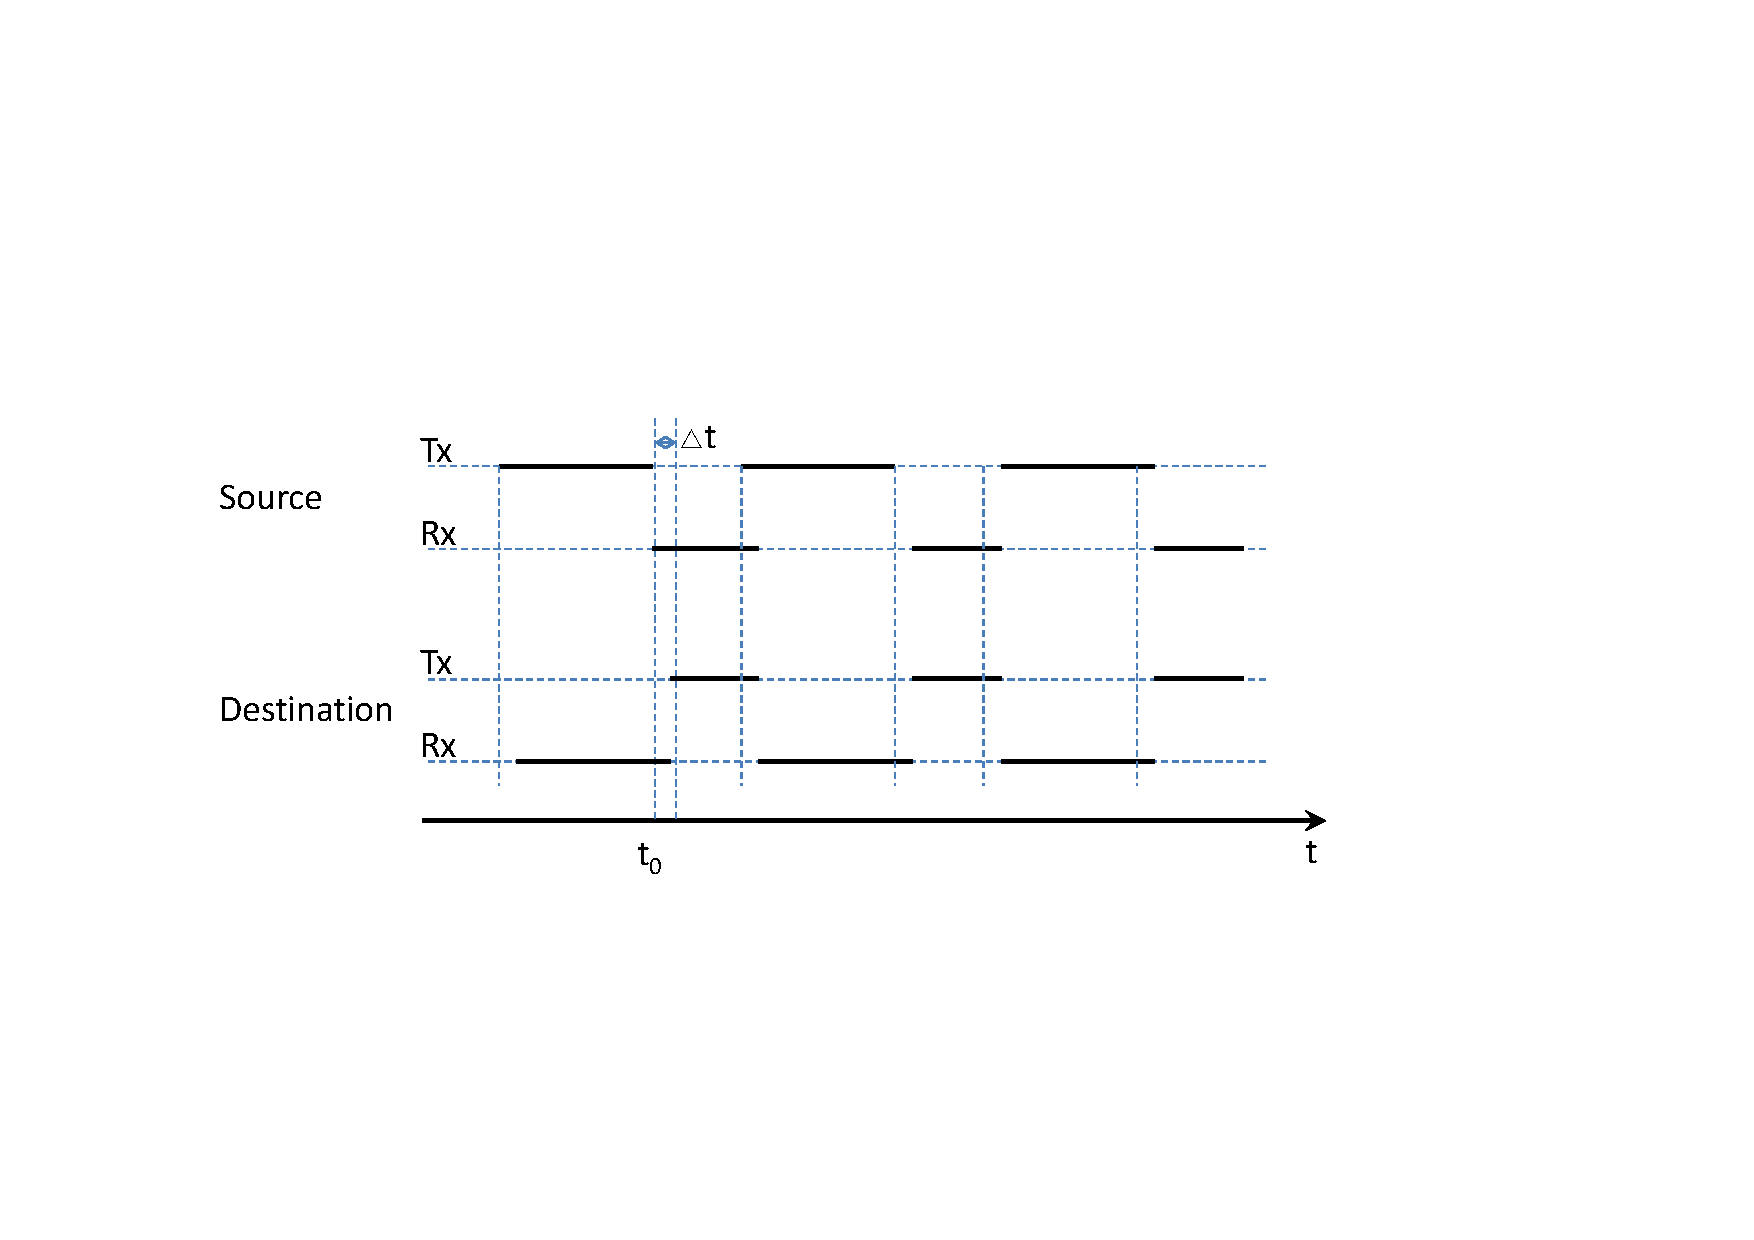
\includegraphics[width=160mm]{TDDoneWayAdjustment.pdf}}
    \caption{Example of one-way TDD timing adjustment. The source adjusts according the data sent from the destination.}
    \label{fig:TDDoneWayAdjustment}
  \end{center}
\end{figure}

Now consider the one-way TDD timing adjustment example as shown in Figure \ref{fig:TDDoneWayAdjustment}. Suppose that starting from time $t_0$, the timing of the destination has a $\Delta t$ offset with respect to the source. The synchronization recovers completely within one TDD cycle.

As a result, one-way TDD timing adjustment is the only option, but a natural question is whether the one-way timing adjustment should be conducted in the forward link or the reverse link.

\subsection{TDD Timing Adjustment in Forward Link vs. Reverse Link}
\label{TDDTimingAdjustemntForwardReverse}
Synchronization for TDD totally depends on the timing adjustment. If more than one physical-layer packet is successfully received, the TDD timing adjustment of TDD can be completed because every physical-layer packet contains the ``sub-frames left'' information. The success probability of TDD timing adjustment relies on the link quality. As Figure~\ref{fig:CompetitiveNodeGeometryFinalRound} suggests, the reverse link has much higher SIR than the forward link, and it is therefore much more reliable than the forward link. As a result, the TDD timing adjustment was chosen to be conducted in the reverse link as discussed in Chapter \ref{chap:strategy}.

However, the transmission time of the reverse link is smaller than that of the forward link, because the ultimate goal is to transmit as many packets as possible in the forward link. If the timing offset between the source and destination is larger than the receiving period of the source node, the TDD timing can never be synchronized as shown in Figure \ref{fig:TDDOneWayAdjFailure}.

A potential solution is to let the receiver of the source wait until it receives at least one useful physical-layer packet, but there are two problems. First, there will not be enough time to prepare the burst data. Second, if the reverse link is not good, our radio has no signal in the air during most of the waiting period. Then our competitor can transmit at higher speed.

\begin{figure}[tpb]
  \begin{center}
    \centerline{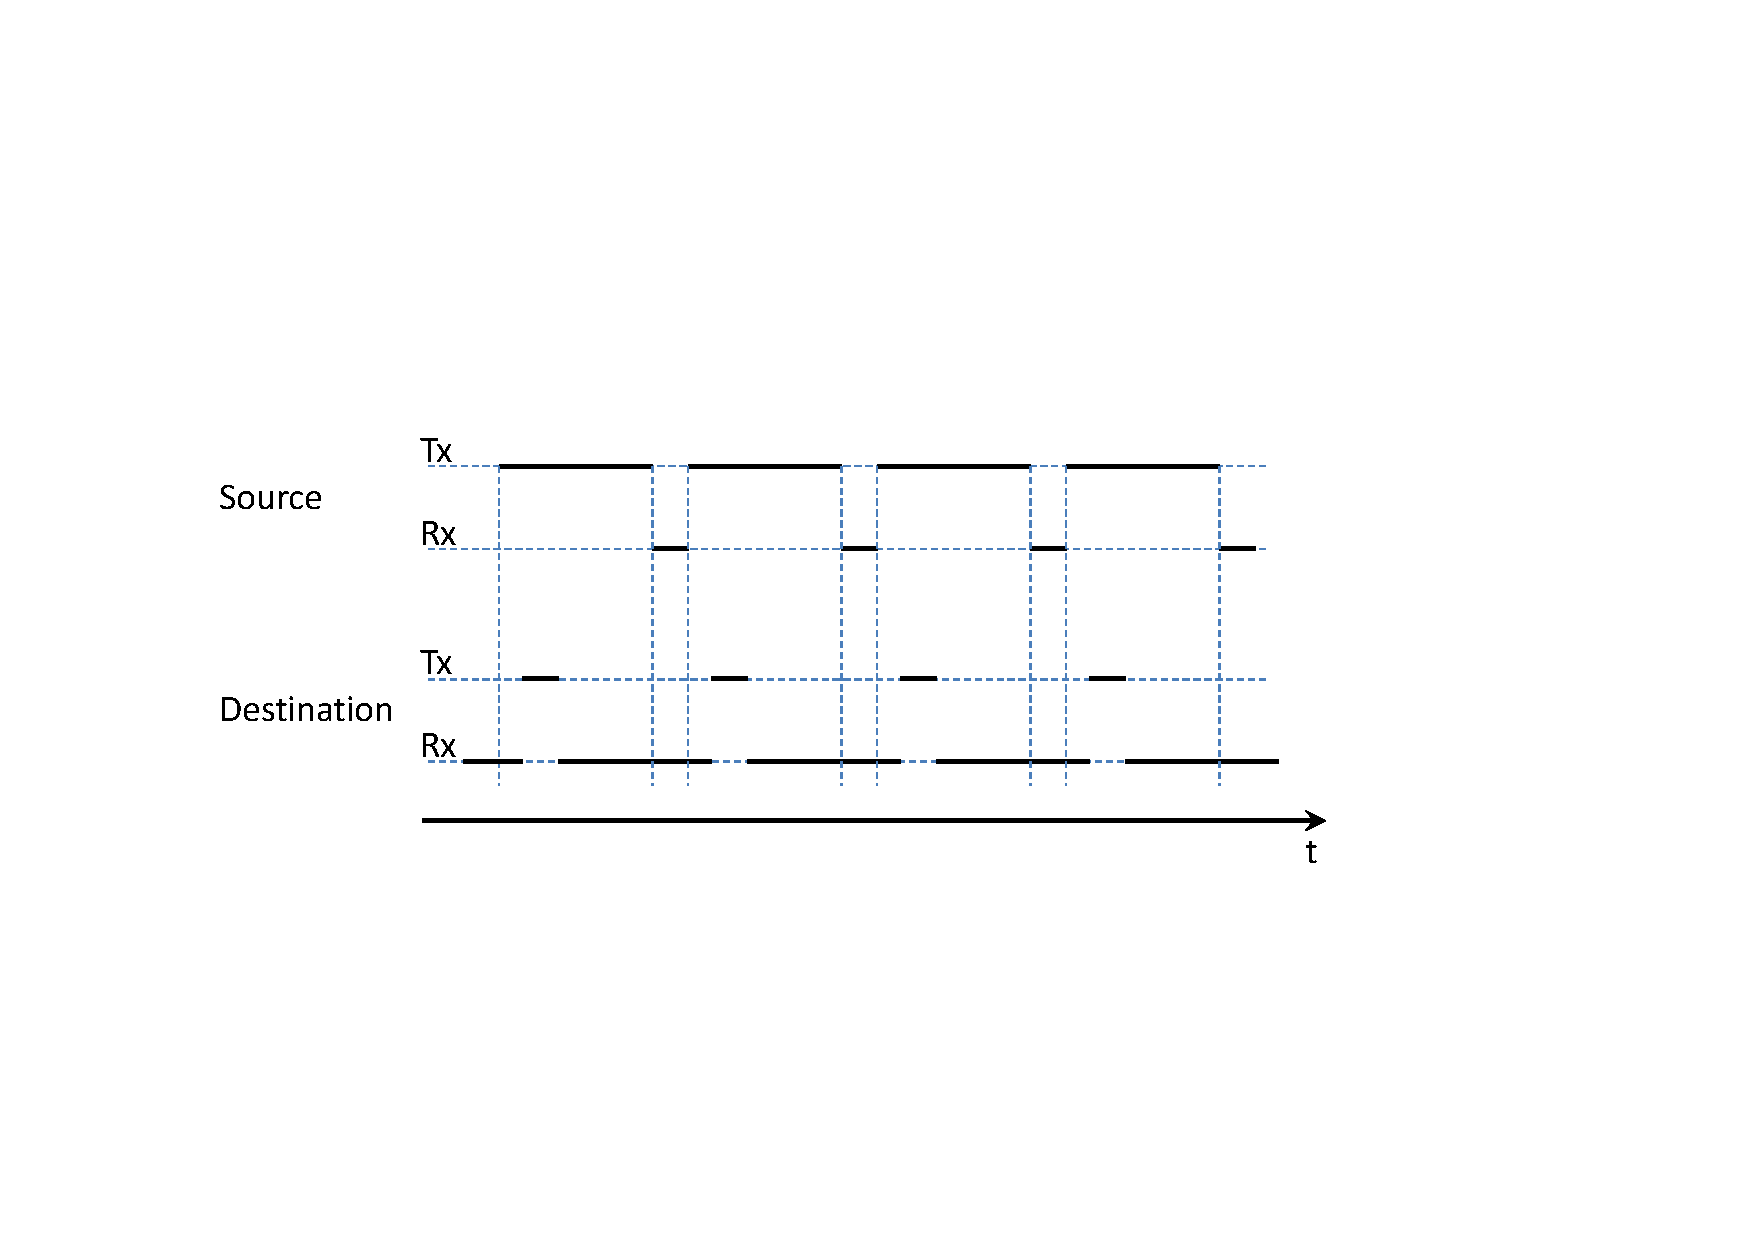
\includegraphics[width=160mm]{TDDOneWayAdjFailure.pdf}}
    \caption{Example of one-way TDD timing adjustment failure in the reverse link. The source adjusts according to the data from the destination.}
    \label{fig:TDDOneWayAdjFailure}
  \end{center}
\end{figure}

This problem can be solved by setting the initial state of the source and destination.
\subsection{Initial State}
There are two potential initial states in TDD system. First, the source and destination will start to transmit in TDD mode immediately after the radios start. The TDD synchronization depends on the one-way TDD timing adjustment. However, as discussed in Section \ref{TDDTimingAdjustemntForwardReverse}, the TDD timing can never be synchronized if the timing offset between the source and destination is larger than the receiving period of the source node as illustrated in  Figure \ref{fig:TDDOneWayAdjFailure}. If the TDD timing adjustment is conducted in the forward link, there will not be a synchronization problem.

The second potential initial state involves the destination starting to transmit in TDD mode initially while the source waits in receiving state for a valid physical-layer packet. After receiving a valid physical-layer packet, the source reverts to its normal TDD mode and adjusts its TDD cycle according to the physical-layer packets received in the reverse link.

For the DARPA Spectrum Challenge, the second initial state was chosen for our system. Figure \ref{fig:TDDflowchart} illustrates the flow graph of the TDD designed. For the TDD used in the DARPA Spectrum Challenge, $m_1=100$ and $m_2=10$.
\begin{figure}[tpb]
  \begin{center}
    \centerline{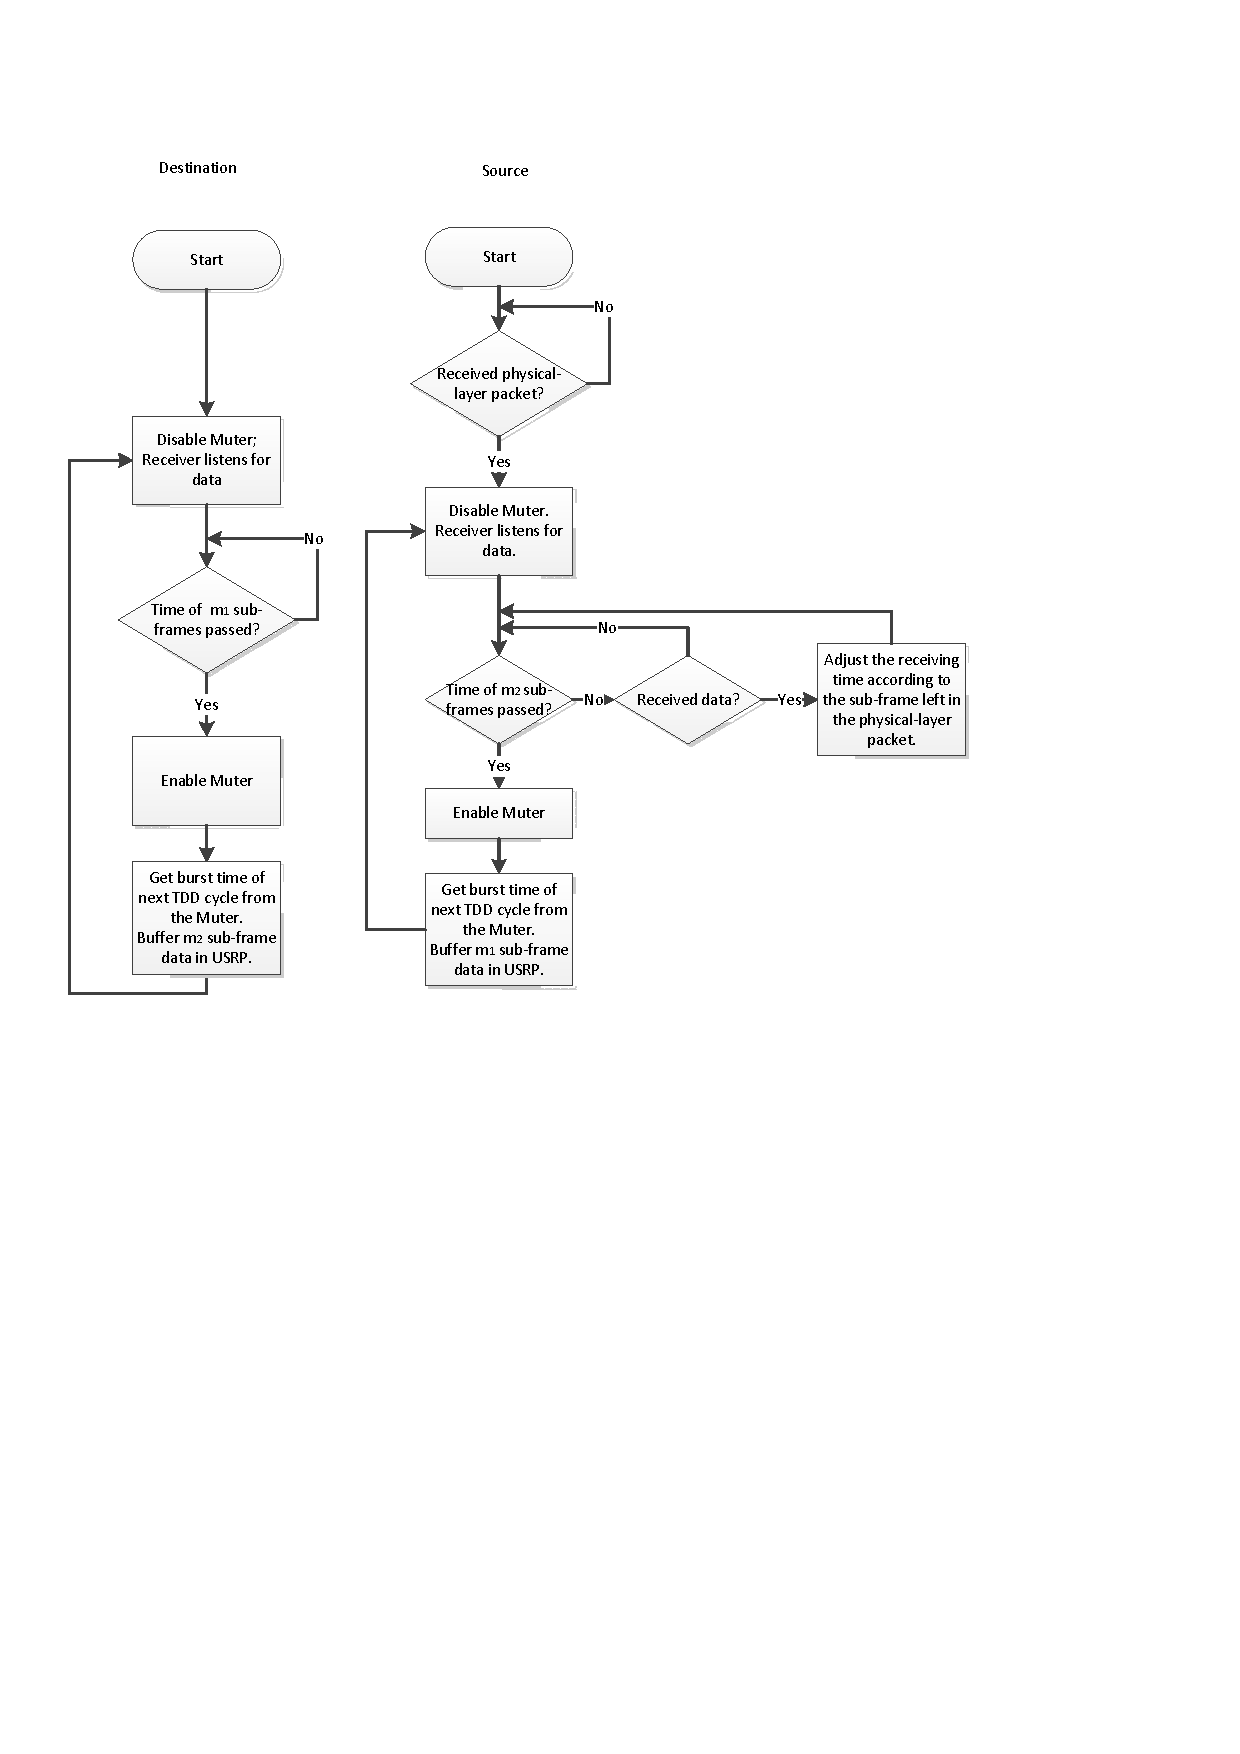
\includegraphics[width=160mm]{TDDflowchart.pdf}}
    \caption{TDD flow graph.}
    \label{fig:TDDflowchart}
  \end{center}
\end{figure}
